\chapter{Time metrology}
Aim of this chapter is to present an issue that will be dealt with in this work.
First a concept of theoretical clock will be presented alongside mathematical tools required
for it description and behavior modelling.
This is followed by a more detailed description of stability analysis which is most prominent
field of science dealing with clock behavior.
After describing theoretical clock models an attention will be given to physical implementation
of clock system with special focus on types of clocks used aboard GPS satellites.
Finally current state of the art in GPS clock bias prediction will be presented.
Intention of writing this chapter was that despite clock modelling and frequency analysis being
well known field readers with computer science might not be familiar with it.
For those well versed in frequency analysis most of this chapter can be safely skipped with 
exception of last section that focuses on state of the art in GPS clock prediction as it 
deals with issues that are more specific do described in this work.
It is important to understand that this chapter do not provide comprehensive knowledge about
described field as due to methodology used in presented work that knowledge it is not required.
For more information about clock modelling and stability analysis Handbook of Frequency Stability
Analysis is suggested as reading.


%====================================================================================================
\section{Physical clock implementation}
\label{sec:physical_clock}

%----------------------------------------------------------------------------------------------------
\subsection{Introduction to physical clock implementation}

%----------------------------------------------------------------------------------------------------
\subsection{Principles of atomic clock design}


%====================================================================================================
\section{Mathematical clock model}
\textbf{FIXME: MAKE ALL EQUATIONS USE SAME NOTATION}
In context of pure mathematical modelling a clock is understood as a function that describes
offset between two given values for a specific point in time. One of those values is referred 
to as the reference clock and it is considered to always return correct time $T_{r}(t)=t$.
It is important to understand that in physical systems value of $t$ is not only inaccessible, as
every measurement instrument have some degree of uncertainty, but do not exists at all.
This is due to time dilatation effect, derived from special theory of relativity, that causes
time to flow differently in systems that move with velocities close to speed of the light.
This issue is dealt with by selecting most precise physical clock available as the reference
clock and modelling difference between it and other clocks, including time dilatation effects,
as their bias.
Main goal of modeling clocks is to retrieve a value of $t$, which is equal to $T_{r}(t)$, based
on value read from given clock $T_{c}(t)$. 
As relation between those clock is fully described by analyzed clock bias 
$b_{c}(t)=T_{r}(t)-T_{c}(t)$ clock model is equivalent to just a bias model.

%----------------------------------------------------------------------------------------------------
\subsection{Discrete and continuous clock models}
There are two possible approaches to mathematical clock modelling, one of them is continuous
clock model that relies on differential equation for description of its behavior.
In this approach clock bias is modeled as :
\begin{equation}
	\label{equ:continous_clock}
	b_{c}(t) = T_{r}(t_{0}) +  \int_{t_{0}}^{t} \varepsilon_{c}(\tau) d\tau ,
\end{equation}
where:
\begin{itemize}
	\item $t$ is the independent time argument,
	\item $b_{c}(t)$ is the clock bias at time $t$,
	\item $t_{0}$ is time at which clock was synchronized with reference ($b_{c}(t_{0})=0$),
	\item $T_{r}(t_{0})$ is value of reference clock at $t_{0}$,
	\item $\varepsilon_{c}(\tau)$ is the normalized frequency offset of a clock.
\end{itemize}
The branch of science that deals with continuous clock modelling is called stability analysis.
In this work no more attention will be given to that approach as due to nature of data as well as
choice of prediction algorithms favour a discrete clock model.
In discrete clock model bias is described as :
\begin{equation}
	\label{equ:discrete_clock}
	b_{c}(i) = T_{r}(i) - T_{c}(i),
\end{equation}
where $i \in \mathbb{N}$ is the number of measurement.
One of main differences between continuous and discrete models is that in latter case bias is 
considered only as a difference between two individual measurements where in case of 
continuous model all differences starting from synchronization are taken into account.
Another important change is that in discrete model clock is a function $\mathbb{N} \to \mathbb{R}$
instead of $\mathbb{R} \to \mathbb{R}$ like it was in case of continuous model. 
This requires redefinition of reference clock from $T_r{t}=t$ into:
\begin{equation}
	\label{equ:discrete_reference}
	T_{r}(i) = \Delta T_r i,
\end{equation}
where $\Delta T_r$ is the measurement period of reference clock.
In such model $T_{r}$ as well as $T_{c}$ are time series which means that $b_{c}$ is also one.
This means that methodologies related to time series analysis like \textbf{TODO : LIST METHODS}
can be used.
Usually clocks are modelled as a linear combination of several deterministic and stochastic 
components as shown on Figure \ref{fig:clocks_example}. 
\begin{figure}[htb] 
\label{fig:clocks_example}
\centering
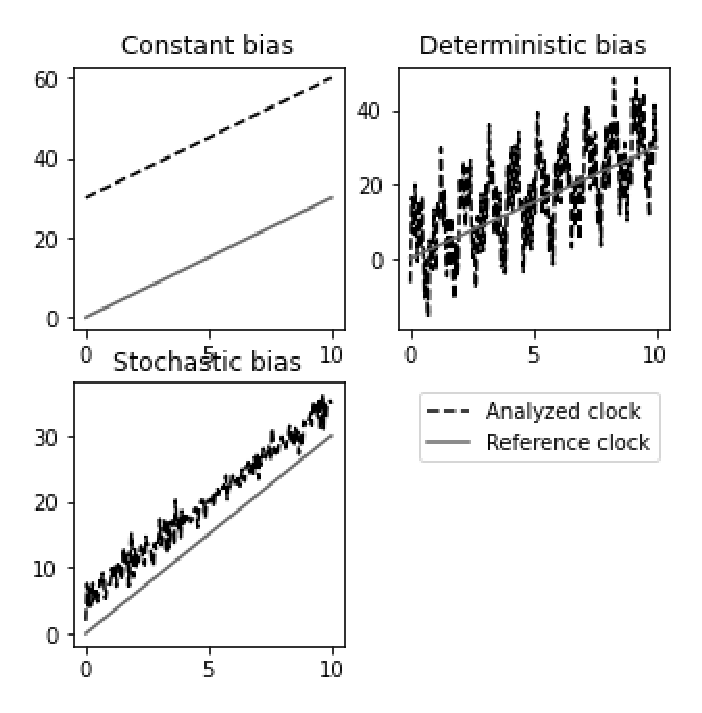
\includegraphics[width=0.5\textwidth]{figures/bias_examples}
\caption{Example of clock readouts depending of nature of their bias}
\end{figure}
More information on exact clock and noise models will be given in following sections.

%----------------------------------------------------------------------------------------------------
\subsection{Basic clock model}
Basic clock model is a deterministic representation of clock as a second-order linear differential
equation.
\begin{equation}
	\label{equ:basic_clock}
	\ddot{x}(t)=z(t).
\end{equation}
Solution to that equation is
\begin{equation}
	\label{equ:basic_clock_solved}
	x(t)=x_{0}+y_{0}\tau+0.5z_{0}\tau^{2},
\end{equation}
where:
\begin{itemize}
	\item $x(t)$ is clock measurement at time $t$, also called time-offset or bias,
	\item $y(t)$ is fractional frequency offset,
	\item $z(t)$ is fractional frequency drift,
	\item $\tau$ is time difference defined as $\tau = t-t_{0}$.
\end{itemize}
Values $x_{0}$, $y_{0}$, $z_{0}$ refer to initial state of model at $t=t_{0}$.
Because frequency stability of clock degrades over time, as a result of ageing of physical 
components that they consist of, fractional frequency drift is sometimes called clock 
ageing parameter.
In this work $z(t)$ will be also referred to as the linear frequency drift. This terminology
was applied as in case of data used in this research there is a observable deterministic 
first order frequency drift behaviour.

%----------------------------------------------------------------------------------------------------
\subsection{Oscillator noise model}
Basic clock model is limited as it allows only for description of simple deterministic systems 
while real life implementations of clock are complex system with both deterministic and 
stochastic components. 
As described in section \ref{sec:physical_clock} of this chapter central element of every clock,
including atomic clocks, is an oscillator. That is why to create a more complex clock models 
an oscillator noise model must be created.
Role of this model is to derive a clock frequency and phase form an actual physical observation 
which in case of an atomic clock is voltage signal.
Equation describing voltage level on quartz oscillator, which is type of oscillator present in
atomic clocks, can be described by an equation:
\begin{equation}
	\label{equ:quartz_voltage}
	U(t)=(U_{0}+\epsilon(t))sin(2\pi \nu_{0}t + \phi(t)),
\end{equation}
where:
\begin{itemize}
	\item $U_{0}$ is peak voltage amplitude,
	\item $\nu_{0}$ is nominal frequency,
	\item $\phi(t)$ represents random phase deviations,
	\item $\epsilon(t)$ represents random amplitude deviations.
\end{itemize}
Since variation in signal amplitude do not influence measurements of signal frequency, save for
extreme cases where it drops so low that signal peak is not registered, it can be ignored in 
equation used for frequency stability analysis.
This means that equation actually used is:
\begin{equation}
	\label{equ:quartz_voltage_simplified}
	U(t)=U_{0}sin(2\pi \nu_{0}t + \phi(t)).
\end{equation}
Instantaneous clock frequency can be defined as the time derivative of the phase as demonstrated
on following equation:
\begin{equation}
	\label{equ:inst_frequency}
	\nu(t) = \nu_{0}+ \frac{1}{2\pi} \frac{d\phi}{dt},
\end{equation}
where $\frac{d\phi}{dt}$ represents instantaneous frequency offset.
The performance of the clock oscillator is determined by the frequency stability and not 
total frequency and the value of frequency offset is usually small in relation to measured.
Because of that it is more meaningful to describe clock stability with normalized, or fractional,
frequency as described in equation:
\begin{equation}
	\label{equ:normalized_frequency}
	y(t) = \frac{\nu(t)-\nu_{0}}{\nu_{0}} = \frac{dx}{dt}
\end{equation}
where
\begin{equation}
	\label{equ:what_is_time_offset}
	x(t) = \frac{\phi(t)}{2\pi \nu_{0}}
\end{equation}
is bias described in the units of time.


%----------------------------------------------------------------------------------------------------
\subsection{Standard clock model}
Standard clock model is most commonly used mathematical description of the clock that models it as
driven by an oscillator that is in periodic motion around a nominal frequency.
It models how precise clocks are subject to both deterministic bias as well as stochastic 
frequency fluctuations.
Mathematically the standard clock model is represented as a first order stochastic differential
equation . Two state model, with states representing time offset and fractional frequency offset
is described by Galleani. However in this work more focus will be given to three state model 
with states representing clock bias, fractional frequency offset and frequency drift.
This model was presented by Chaffee in 1987 and is described as :
\begin{equation}
	\label{equ:three_state_clock}
	\left[ \begin{array}{c} dx(t)\\ dy(t)\\ dz(t) \end{array} \right] =
	\left[ \begin{array}{ccc} 0& 1& 0\\ 0& 0& 1\\ 0& 0& 0 \end{array} \right]
	\left[ \begin{array}{c} x(t)\\ y(t)\\ z(t) \end{array} \right] dt +
	\left[ \begin{array}{c} d\epsilon(t)\\ d\zeta(t)\\ d\eta(t) \end{array} \right] 
\end{equation}
which is using matrix notation can be described as :
\begin{equation}
	\label{equ:clock_matrix}
	dX(t) = AX(t) +dB(t).
\end{equation}
In those equations $x(t)$, $y(t)$ and $z(t)$ are respectively clock bias, fractional frequency and
fractional frequency drift while $\epsilon(t)$ $\zeta(t)$ and $\eta(t)$ are zero mean Gaussian
white noise processes. They are described as:
\begin{itemize}
	\item $\epsilon(t)$ is white frequency modulation (WFM),
	\item $\zeta(t)$ is random walk frequency modulation (RWFM),
	\item $\eta(t)$ is random run frequency modulation (RRFM).
\end{itemize}
With this it is clear that in matrix notation $X$ is clock state matrix, $A$ is state transition
matrix while $B$ is random noise matrix.
As this work do not focuses on stochastic differential equations only a solution for the equation
\ref{equ:three_state_clock} will be shown, for those more interested in how it was calculated 
more basic literature on topic of SDE is suggested.
\begin{equation}
	\label{equ:clock_solved}
	X(t) = \Phi(t,t_{0})X(t_{0}) + \int^{t}_{t_0}\Phi(t,\tau)dB(\tau),
\end{equation}
where
\begin{equation}
	\label{equ:what_is_phi}
	\Phi(t,t_{0}) = e^{At-t_{0}} = \sum^{\infty}_{0}\frac{(A(t-t_{0}))^2}{n!},
\end{equation}
and $X_{0}$ is the initial condition.
If $X(t_{0})$ is assumed to be a non-random constant then $X(t)$ is a Gaussian process with 
stationary increments and clock bias at time $t$ can be calculated with equation:
\begin{equation}
	\label{equ:bias_final}
	x(t)=x(t_{0}) + y(t-t_{0}) + z(t_{0})\frac{(t-t_{0})^2}{2} + \int^{t}_{t_{0}}d\epsilon(\lambda)
	+ \int^{t}_{t_{0}}(t-\lambda)d\zeta(\lambda) 
	+ \int^{t}_{t_{0}}\frac{(t-\lambda)^2}{2}d\eta(\lambda),
\end{equation}
where the integrals represent noise processes and terms above 2 are excluded.

%====================================================================================================
\section{Stability analysis}
Quality of an oscillator is determined by its frequency stability over time. 
As both phase and frequency influence clock readouts so stability analysis must focus on both.


%----------------------------------------------------------------------------------------------------
\subsection{Allan variance}
Allan variance, also know as the two-sample variance, is the default descriptive statistic
for time and frequency measurements.
This is because standard variance is not suitable for modelling non stationary processes.
The Allan variance is formally adopted as a standard for characterising and reporting instabilities
in phase, frequency or amplitude measurements in time domain.
Allan variance is an infinite time average of the square of the difference of two fractional
frequency measurements:
\begin{equation}
	\label{equ:allan_first}
	\sigma^{2}_{y}(\tau)=0.5\langle (\hat{y}_{k+1}-\hat{y}_k)^{2}  \rangle,
\end{equation}
where $\langle \rangle$ denotes the infinite time average operator while $\hat{y}_k$ is a 
frequency at time $t_{k}$. Hat over variable indicates that value is estimated from phase
measurements with following equation:
\begin{equation}
	\label{equ:y_hat}
	\hat{y}_{k}=\frac{1}{\tau}\int^{t_{k+1}}_{t_{k}}y(t)dt =
	\frac{x(t_{k+1})-x(t_{k})}{\tau},
\end{equation}
In real world application Allan variance is calculated basing on the set of a measurements which
is always a finite set. Therefore as data worked upon is finite and discrete in time domain 
Allan variance can be described as:
\begin{equation}
	\label{equ:allan_discrete}
	\sigma^{2}_{y}(\tau) = \frac{1}{2(M-1)}\sum^{M-1}_{k=1}(\hat{y}_{k+1}-\hat{y}_{k})^2,
\end{equation}
where $M$ denotes number of measurements.
By substituting selected values in equation \ref{equ:allan_discrete} Allan variance can be
described as a function of phase or time offset
\begin{equation}
	\label{equ:allan_discrete2}
	\sigma^{2}_{y}(\tau) = \frac{1}{2(M-1)\tau^{2}}\sum^{M-1}_{k=1}(x_{k+2}-2x_{k+1}+x_{k})^2.
\end{equation}
Even better estimation of Allan variance can be achieved by calculating what it is called a
overlapping Allan variance. This is because it forms all possible overlapping combinations of
available data
\begin{equation}
	\label{equ:overlapping_allan}
	\sigma^{2}_{y}(\tau) = \frac{1}{2(N-2m)\tau^{2}}\sum^{N-2m}_{k=1}(x_{k+2m}+2x_{k+m}+x_{k})^2.
\end{equation}
As overlapping Allan variance provides better results than its basic version in most cases 
literature dealing with stability analysis will use term Allan variance to refer to it 
overlapping version unless specified otherwise.
There is also one more variant called modified Allan variance that unlike all previous examples
can distinguish between WPM and FPM.
In term of phase modified Allan variance is described as:
\begin{equation}
	\label{equ:modified_allan}
	\sigma^{2}_{y}(\tau)=\frac{1}{2m^{2}\tau^{2}(N-3m+1)\tau^{2}}\sum^{N-3m+1}_{j=1}(
	\sum^{j+m-1}_{k=j}(x_{k+2m}-3x_{k+m}+x_{k})^2)
\end{equation}

%--------------------------------------------------------------------------------------------------
\subsection{Hadamard variance}
Hadamard variance was derived from the Hadamard transform for use in stability analysis by 
Baugh.  As the Allan variance describes a second-order phase variation so Hadamard variance 
describes third-order phase variation.
Unlike Allan variance Hadamard variance is insensitive to linear frequency drift, this is 
especially important in context of this work as rubidium clocks used in GPS satellites have a 
prominent linear drift.
As with Allan variance the overlapping version of equation is used as default:
\begin{equation}
	\label{equ:overlapping_hadamard}
	\sigma^{2}_{H} = \frac{1}{6(N-3m)\tau^2}
	\sum^{N-3m}_{k=1}(x_{k+3m}-3x_{k+2m}+3x_{k+m}-x+{k})^{2}
\end{equation}

%====================================================================================================
\section{Modeling noise}


%----------------------------------------------------------------------------------------------------
\subsection{White phase modulation noise}

%----------------------------------------------------------------------------------------------------
\subsection{Flicker phase modulation noise}

%----------------------------------------------------------------------------------------------------
\subsection{White frequency modulation noise}

%----------------------------------------------------------------------------------------------------
\subsection{Flicker frequency modulation noise}

%----------------------------------------------------------------------------------------------------
\subsection{Random walk frequency modulation noise}

%----------------------------------------------------------------------------------------------------
\subsection{Oscilator noise as linear combination of power-law noises}

%----------------------------------------------------------------------------------------------------
\subsection{Sources of noise specific to orbital clocks}


%====================================================================================================
\section{State of the art in GPS clock bias prediction}

%----------------------------------------------------------------------------------------------------
\subsection{Time references in GPS}

%----------------------------------------------------------------------------------------------------
\subsection{Satellite broadcast polynomial}

%----------------------------------------------------------------------------------------------------
\subsection{IGU products}
